\section{Automata Web-Ebay}
\subsection{ Descripci\'on del programa}
\justify
El siguiente programa reconoce todas las palabras que contengan web o ebay,esto se realizar por medio de un automata finito determinista, podr\'a reconocer las palabras solo en textos en ingl\'es.\\
Consta de un modo autom\'atico y manual, ademas se podr\'a visualizar el diagrama del aut\'omata.\\
El programa guarda todas las palabras que encontr\'o y las guarda en un archivo de texto indicando el numero de fila y palabra en la que se encuentra.\\
\subsection{C\'odigo}
El c\'digo utilizado para la resoluci\'on del problema se muestra a continuaci\'on:\\

C\'odigo: webay.py
\lstset{language=Python, breaklines=true, basicstyle=\footnotesize}
\begin{lstlisting}[frame=single]
def automataWebay(caracter,estado,archivo):
	if(estado==0):
		estado=estadoCero(caracter,archivo)
	elif(estado==1):
		estado=estadoUno(caracter,archivo)
	elif(estado==2):
		estado=estadoDos(caracter,archivo)
	elif(estado==3):
		estado=estadoTres(caracter,archivo)
	elif(estado==4):
		estado=estadoCuatro(caracter,archivo)
	elif(estado==5):
		estado=estadoCinco(caracter,archivo)
	elif(estado==6):
		estado=estadoSeis(caracter,archivo)
	elif(estado==7):
		estado=estadoSiete(caracter,archivo)

	return estado

def estadoCero(caracter,archivo):
	if (caracter=='w'):
		archivo.write('q0--w-->q1\t')
		return 1
	elif (caracter=='e'):
		archivo.write('q0--e-->q4\t')
		return 4
	else:
		archivo.write('q0--%s-->q0\t' %caracter)
		return 0

def estadoUno(caracter,archivo):
	if(caracter=='w'):
		archivo.write('q1--w-->q1\t')
		return 1
	elif(caracter=='e'):
		archivo.write('q1--e-->q2\t')
		return 2
	else:
		archivo.write('q1--%s-->q0\t' % caracter)
		return 0

def estadoDos(caracter,archivo):
	if(caracter=='w'):
		archivo.write('q2--w-->q1\t')
		return 1
	elif(caracter=='e'):
		archivo.write('q2--e-->q4\t')
		return 4
	elif(caracter=='b'):
		archivo.write('q2--b-->q3\t')
		return 3
	else:
		archivo.write('q2--%s-->q0\t' % caracter)
		return 0

def estadoTres(caracter,archivo):
	if(caracter=='w'):
		archivo.write('q3--w-->q1\t')
		return 1
	elif(caracter=='e'):
		archivo.write('q3--e-->q4\t')
		return 4
	elif(caracter=='a'):
		archivo.write('q3--a-->q6\t')
		return 6
	else:
		archivo.write('q3--%s-->q0\t' % caracter)
		return 0

def estadoCuatro(caracter,archivo):
	if(caracter=='w'):
		archivo.write('q4--2-->q1\t')
		return 1
	elif(caracter=='e'):
		archivo.write('q4--e-->q4\t')
		return 4
	elif(caracter=='b'):
		archivo.write('q4--b-->q5\t')
		return 5
	else:
		archivo.write('q4--%s-->q0\t' % caracter)
		return 0

def estadoCinco(caracter,archivo):
	if(caracter=='w'):
		archivo.write('q5--w-->q1\t')
		return 1
	elif(caracter=='e'):
		archivo.write('q5--e-->q4\t')
		return 4
	elif(caracter=='a'):
		archivo.write('q5--a-->q6\t')
		return 6
	else:
		archivo.write('q5--%s-->q0\t' % caracter)
		return 0

def estadoSeis(caracter,archivo):
	if(caracter=='w'):
		archivo.write('q6--w-->q1\t')
		return 1
	elif(caracter=='e'):
		archivo.write('q6--e-->q4\t')
		return 4
	elif(caracter=='y'):
		archivo.write('q6--y-->q7\t')
		return 7
	else:
		archivo.write('q6--%s-->q0\t' % caracter)
		return 0

def estadoSiete(caracter,archivo):
	if(caracter=='w'):
		archivo.write('q7--w-->q1\t')
		return 1
	elif(caracter=='e'):
		archivo.write('q7--e-->q4\t')
		return 4
	else:
		archivo.write('q7--%s-->q0\t' % caracter)
		return 0

\end{lstlisting}
\vspace{1.5cm}
C\'odigo:main.py

\lstset{language=Python, breaklines=true, basicstyle=\footnotesize}
\begin{lstlisting}[frame=single]
import webay
import diagrama

def menu():
    try:
        opcion=input('\t\t-------------WEBAY------------\n1.-Modo manual\n2.-Leer texto\n3.-Diagrama\n4.-Salir\nElija una opcion: ')
        opcion=int(opcion)
    except:
        print('\nIntroduzca una opcion correcta\n')

    return opcion

def IniciarArchivo():
    archivo=open("Palabras.txt","w")
    archivo.close
    archivoH=open("Historia.txt","w")
    archivo.close

def AbrirArchivo():
    try:
        archivo=open("Palabras.txt","a")
    except:
        print("\nError al abrir el archivo")
        exit()
    return archivo

def AbrirHistoria():
    try:
        archivo=open("Historia.txt","a")
    except:
        print("\nError al abrir el archivo")
        exit()
    return archivo

def escribir(archivo,palabra_aux,no_palabra,no_fila):
    archivo.write("Palabra: "+palabra_aux+" Numero de palabra: "+str(no_palabra)+" Numero de fila: "+str(no_fila))
    archivo.write("\n")


def Evaluar(texto):
    archivo=AbrirArchivo()
    historia=AbrirHistoria()
    palabra_aux=''
    final=False
    estado=0
    no_palabra=1
    no_fila=1

    historia.write("\n\n\n\n")
    for caracter in texto:
        caracter=caracter.lower()
        estado=webay.automataWebay(caracter,estado,historia)
        if(estado==3 or estado==7):
            final=True
        if(caracter=='\n'):
            if(final):
                escribir(archivo,palabra_aux,no_palabra,no_fila)
                historia.write("\n")
                palabra_aux=''
                final=False
            else:
                palabra_aux=''
            no_palabra=1
            no_fila=no_fila+1
            continue
        if (caracter==' '):
            if(final):
                escribir(archivo,palabra_aux,no_palabra,no_fila)
                historia.write("\n")
                palabra_aux=''
                final=False
            else:
                palabra_aux=''
            no_palabra=no_palabra+1

            continue
        palabra_aux=palabra_aux+caracter
    if(final):
        no_palabra=no_palabra+1
        escribir(archivo,palabra_aux,no_palabra,no_fila)
        historia.write("\n")

    archivo.close
    historia.close
def leer_Archivo():
    try:
        archivo=open("archivo.txt","r")
        texto=str(archivo.read())
    except:
        print("\nError al abrir el archivo")
        exit()
    return texto

def main():
    IniciarArchivo()
    while True:
        eleccion=menu()
        if(eleccion==1):
            texto=input("Introduzca un pequenio texto: ")

            Evaluar(texto)
            print("Evaluacion terminada, cheque el archivo de texto")
            while True:
                reop=input("Desea regresar al menu\n1.-Si\n2.-No\nEleccion: ")
                if(reop=='1'):
                    break
                elif(reop=='2'):
                    exit()
                else:
                    continue
        elif(eleccion==2):
            texto=leer_Archivo()

            Evaluar(texto)
            print("Evaluacion terminada, cheque el archivo de texto")
            while True:
                reop=input("Desea regresar al menu\n1.-Si\n2.-No\nEleccion: ")
                if(reop=='1'):
                    break
                elif(reop=='2'):
                    exit()
                else:
                    continue
        elif(eleccion==3):
            diagrama.mostrarDiagrama()
            while True:
                reop=input("Desea regresar al menu\n1.-Si\n2.-No\nEleccion: ")
                if(reop=='1'):
                    break
                elif(reop=='2'):
                    exit()
                else:
                    continue
        elif(eleccion==4):
            exit()
        else:
            continue
main()


\end{lstlisting}
\vspace{1.5cm}
C\'odigo:diagrama.py

\lstset{language=Python, breaklines=true, basicstyle=\footnotesize}
\begin{lstlisting}[frame=single]
	sjdkasjdkasjdksa
\end{lstlisting}

\newpage

\subsection{Pruebas}
A continuaci\'on se mostraran algunas im\'agenes capturadas al momento de ejecutar el programa, dichas im\'agenes mostraran los resultados obtenidos.\\
\vspace{1.0cm}
Para el modo manual:\\
\begin{figure}[H]
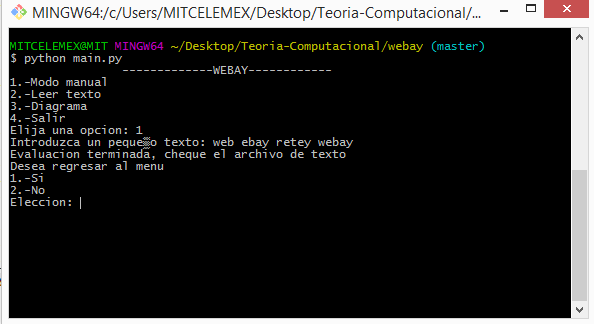
\includegraphics[width=\textwidth, height=7cm]{ModoManualWebay.png}
\label{fig:manual_webay}
\caption{Palabras de prueba: web ebay retey webay}
\end{figure}

\begin{figure}[H]
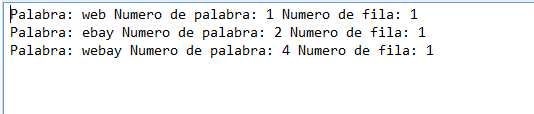
\includegraphics[width=\textwidth, height=7cm]{ArchivoWebay.png}
\label{fig:manualtexto_alfabeto}
\caption{Salida del archivo de palabras encontradas}
\end{figure}

\begin{figure}[H]
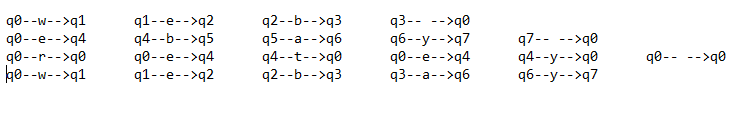
\includegraphics[width=\textwidth, height=7cm]{HistoriaWebay.png}
\label{fig:manualnuevoconteo_alfabeto}
\caption{Historia de la evaluaci\'on del aut\'omata}
\end{figure}

Para el modo de lectura de un archivo:\\
\begin{figure}[H]
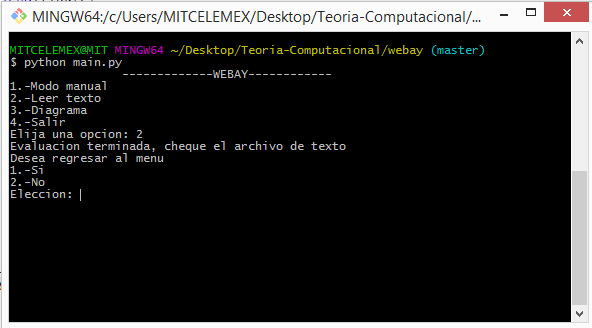
\includegraphics[width=\textwidth, height=7cm]{ModoAutomaticoWebay.png}
\label{fig:auto_alfabeto}
\caption{Lectura de un texto con palabras WEB}
\end{figure}

\begin{figure}[H]
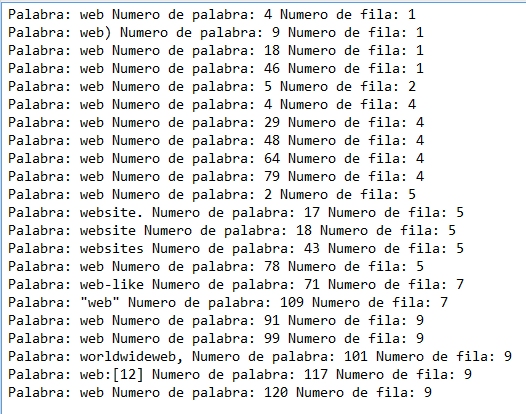
\includegraphics[width=\textwidth, height=7cm]{ArchivoTextoWebay.png}
\label{fig:autotexto_alfabeto}
\caption{Palabras encontradas del texto}
\end{figure}

\begin{figure}[H]
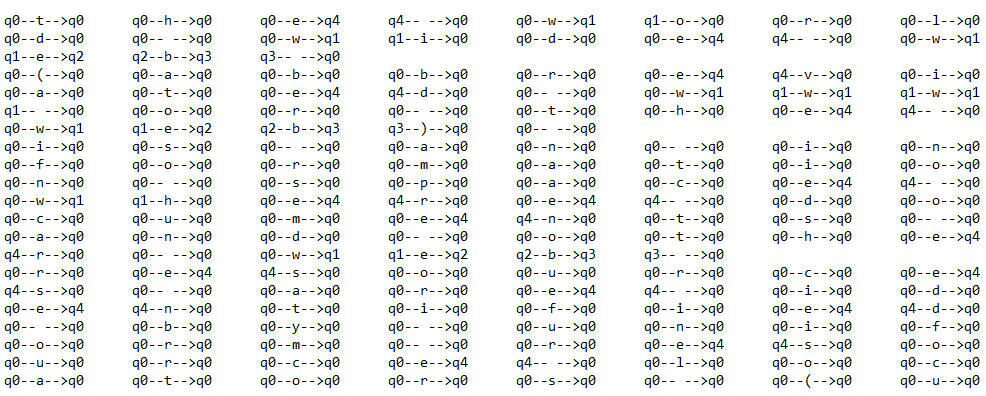
\includegraphics[width=\textwidth, height=7cm]{HistoriaWebayA.png}
\label{fig:manualnuevoconteo_alfabeto}
\caption{Historia de la evaluaci\'on del aut\'omata}
\end{figure}

%\begin{figure}[H]
%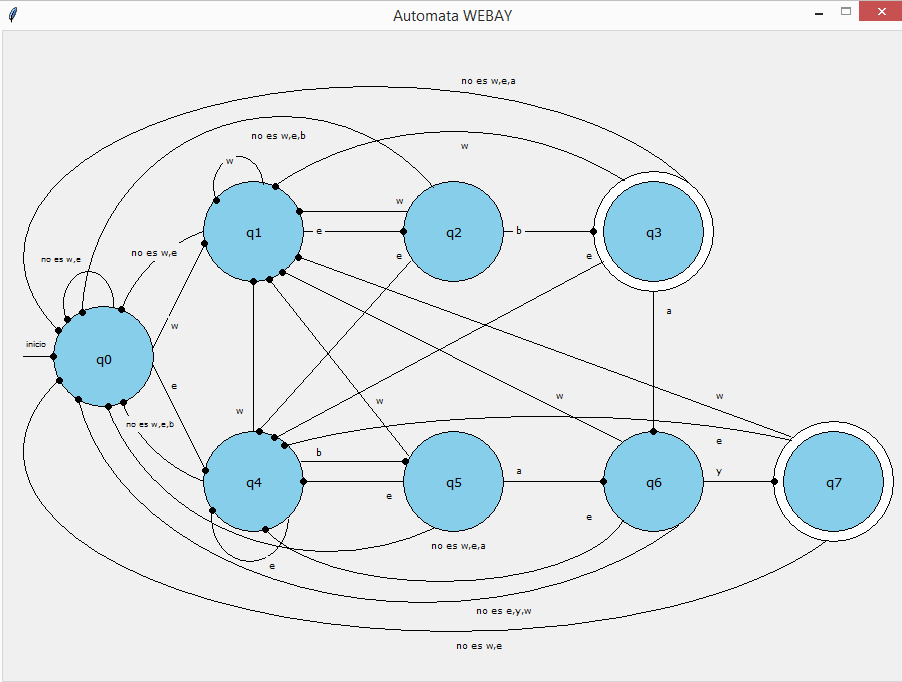
\includegraphics[width=\textwidth, height=7cm]{DiagramaWebay.png}
%\label{fig:manualnuevoconteo_alfabeto}
%\caption{Diagrama del aut\'omata}
%\end{figure}

\newpage

